\chapter{Økonomi}
\section{Indledning}
Eksistensberettigelse for telesundhed – økonomisk besparelse og effektivisering, men er virkeligheden også sådan? Det vil der blive set nærmere på.

Økonomiafsnittet har til formål at belyse omkostningerne ved henholdsvis fysisk hjemmepleje og virtuel hjemmepleje i Favrskov Kommune, og derefter pointere økonomiske forskelle mellem de to scenarier ved hjælp af en ressourceopgørelse.\\ \\
Følgende spørgsmål ønskes besvaret i økonomiafsnittet:
\begin{itemize}
	\item Hvilke økonomiske konsekvenser medfører implementering af telesundhed?
	\item Er der økonomisk gevinst ved at implementere videoopkald, som erstatning for fysiske besøg i Favrskov Kommune?
\end{itemize}

\section{Metode}
Gennem møder med Appinux, Netplan Care og Favrskov Kommune er det nødvendige udstyr for at kunne implementere telesundhed – herunder virtuel hjemmepleje – blevet identificeret.\\
Der er tilegnet informationer om diverse omkostninger ved dette udstyr, samt yderligere omkring arbejdsgange i Favrskov Kommune. 
I tilfælde af mangel på konkret information fra Favrskov Kommune angående specialaftale med Appinux, omfang af målgruppe, tidsbesparelser ved virtuel hjemme pleje kontra fysiske besøg mv., har det været nødvendigt at lave antagelser herom. Antagelserne bygger på vejledende informationer fra Favrskov Kommune.\\
Priserne for Appinux’ løsning er vejledende og ikke nødvendigvis gældende for Favrskov kommune. Det skyldes, at priserne opgivet af Appinux blot er liste priser, og der tages ikke højde for særlige tilbud.\\
Yderligere økonomiske konsekvenser er forsøgt klarlagt gennem en søgning af studier omhandlende videobaserede telesundheds løsninger for hjemmepleje på følgende fem databaser: PubMed, Embase, CINAHL, Cochrane Libary og Google Scholar. Google i al almindelighed er ligeledes benyttet til at samle generel information om telesundhed. 


\section{Resultater}
\subsection{Omkostninger ved implementering og drift af Appinux' løsning}
\subsubsection{Opstartsomkostninger}
Opstartsomkostningerne for Appinux’ telesundhedsløsning med skærmopkald ses på nedenstående figur 1(AA3). Der er vigtigt at pointere, at indkøb af tablets til selve skærmopkaldende ikke er inddraget i figur 1, da den udelukkende belyser opstartsomkostningerne for Appinux’ løsning.

\begin{figure}[H]
	\centering
	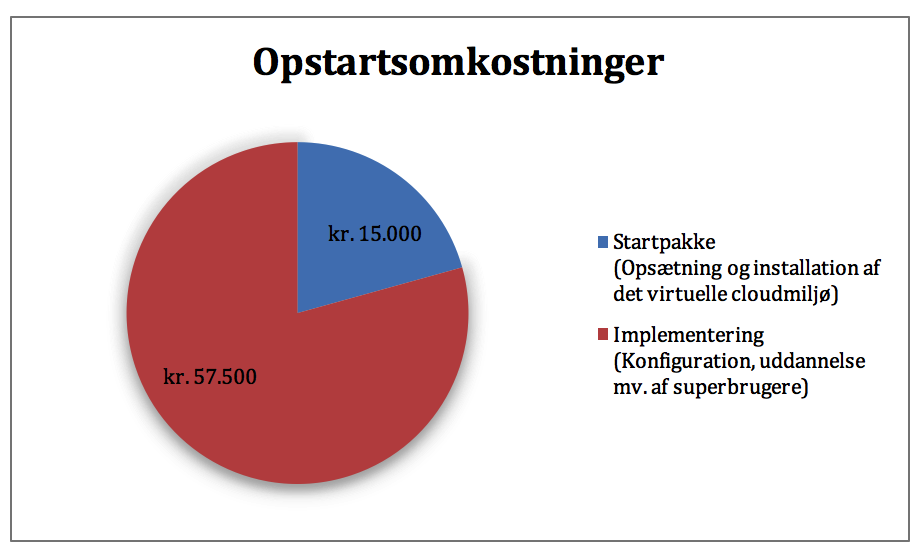
\includegraphics[width=1\textwidth]{Figurer/Snip20160504_26}
	\caption{Opstartsomkostninger for skærmopkald. INDSÆT REFERENCE – MICHAEL ELLEGAARD FRA APPINUX!}
\end{figure}

Appinux tilbyder ikke tablets som en del af deres løsning, og det har ikke været muligt, at indhente informationer og/eller anbefalinger fra Appinux angående tablets, der skal benyttes til skærmopkald.(AA4)
Favrskov Kommune har dog informeret omkring deres indkøb af tablets og covers til brug af netop Appinux’ løsning. 
Tabel 1 tager udgangspunkt i Favrskov Kommunes estimering om, at 25 tablets og covers er tilstrækkeligt med det nuværende potentiale for virtuel hjemmepleje. Prisen ses i tabel X. (AA5) 

\begin{table}[H]
	\caption{Tabel over indkøb af tablets i Favrskov Kommune.}
	\centering
	\label{tab:tabelindkoeb}
	\begin{tabular}{|l|l|l|l|}
		\hline
		\textbf{Beskrivelse} & \textbf{Pris} & \textbf{Antal} & \textbf{Samlet udgift}\\ \hline
		Samsung Tab A Tablet + cover & Kr. 2.300,00 pr. sæt & 25 stk. & kr. 57.500\\ \hline
	\end{tabular}
\end{table}
Det nødvendige antal tilgængelige tablets og covers vil afhænge af mængden af brugere. Udover brugerne skal personalet ligeledes være i besiddelse af en tablet for at kunne foretage skærmopkald til borgerne. Det må antages, at der i fremtiden opstår behov for indkøb af flere nye tablets og covers, hvis der tages udgangspunkt i Favrskov Kommunes mål om at have 50 aktive brugere(AA5).
\subsection{Driftsøkonomi}
\subsubsection{Månedligt abonnement}
Favrskov Kommune abonnerer på Appinux’ løsning og betaler en månedlig pris for de tilkøbte moduler. Abonnementet varierer i pris alt efter, hvilke moduler der tilkøbes, og hvor mange brugere, der benytter modulet.\\
Der tages udgangspunkt i Appinux’ løsning for skærmopkald(”Platform – Forløb, Kalender, Video”), da dette modul giver adgang til at udøve virtuel hjemmepleje.
(AA6)

\begin{table}[H]
	\caption{Tabel over indkøb af tablets i Favrskov Kommune.}
	\centering
	\label{tab:tabelmaanedudgift}
	\begin{tabularx}{\textwidth}{|X|X|}
		\hline
		\textbf{Beskrivelse} & \textbf{Udgift}\\ \hline
		Månedligt abonnement ved Appinux 
		(0-75 brugere)
		 & Kr. 139,00 pr. bruger pr. måned\\ 
		\hline
		Månedligt abonnement ved Appinux 
		(76-300 brugere)
		& Kr. 119,00 pr. bruger pr. måned\\ \hline
				Månedligt abonnement ved Appinux 
				(0-500 brugere)
				& Kr. 22.500,00 pr. måned (Prisen er uafhængig af antallet af brugere, så længe det er mellem 0-500)\\ \hline
	\end{tabularx}
\end{table}

\subsubsection{Løn til personale}
Tabel 3 tager udgangspunkt i, at Favrskov Kommune vælger at opdatere systemet hver gang Appinux stiller en opdatering til rådighed, hvilket er én gang i kvartalet. 

\begin{table}[H]
	\caption{Udgift for Favrskov Kommune for at lave systemopdateringer pr. år}
	\centering
	\label{tab:tabelpersonaleudgift}
	\begin{tabularx}{\textwidth}{|X|X|}
		\hline
		Pris pr. år for at teste opdateringer
		& kr. 11.580\\ 
		\hline
	\end{tabularx}
\end{table}
Favrskov Kommune har dog mulighed for at fravælge hver anden opdatering og kun opdatere systemet én gang hvert halve år. På denne måde er det muligt at holde driftsomkostninger nede til et minimum.(AA3) 
\subsubsection{Totalomkostninger}
Der tages ikke højde for løn til personale der foretager skærmopkald og sidder i call-center, uddannelse af superbrugere, forældede tablets, fejlkøb af tablets og en eventuel specialaftale mellem Favrskov Kommune og Appinux.\\ \\

MANGLER FIGUR!!\\ \\

Det ses, at prisen pr. bruger pr. måned varierer efter længden af perioden Favrskov Kommune vælger at benytte skærmopkald. Det skyldes, at opstartsomkostninger forekommer som engangsbetaling, og dermed vil den gennemsnitlige pris pr. bruger pr. måned falde i takt med anvendelsesperioden. 
(AA7 - artikel)
\subsection{Usikkerheder/yderligere omkostninger}
Dette afsnit har til formål at belyse usikkerheder og eventuelle fremtidige omkostninger. 

\subsubsection{Superbrugere}
Favrskov Kommune har 26 superbrugere tilknyttet Appinux’ løsning, hvoraf nogle af dem er tilknyttet virtuel hjemmepleje. Hvert halve år afholder de et fælles superbrugermøde af halvanden times varighed for alle superbrugere. (AA8)\\
Superbrugerne har det generelle ansvar for at oprette/fjerne brugere/kollegaer i systemet, samt andre små opgaver. \\
Dette er ligeledes en omkostning, der skal tages i betragtning ved erhvervelse af virtuel hjemmepleje. Det må antages, at kommunen skal bruge yderligere ressourcer på uddannelse af nye superbrugere i tilfælde af, at personale kvalificeret som superbruger fratræder sin stilling. 
Omkostningen må forventes at variere i forbindelse med antallet af brugere, idet flere brugere kræver mere personale til håndtering af skærmopkald. (AA9).

\subsubsection{Tablets}
Favrskov Kommune købte - ved starten af samarbejdet med Appinux - nogle nye tablets, men de tekniske kvalifikationer var ikke tilstrækkelige til at benytte skærmopkald(AA4), hvorfor efterfølgende indkøb af bedre tablets var nødvendigt.\\
I fremtiden kan der opstå behov for yderligere indkøb af tablets i tilfælde af, at antal brugere overstiger mængden af første portion indkøbte tablets. Ydermere kan ekstra indkøb af tablets forekomme som resultat af defekte tablets.

\subsubsection{Antal brugere}
Figur 2 viser betydningen af antal brugere, idet prisen pr. bruger pr. måned er lavere, hvis flere benytter skærmopkald.\\
Omfanget af brugergruppen har derfor stor betydning for de økonomiske konsekvenser. 

\subsubsection{Ugennemsigtige priser}
Priserne er bygget på listepriser fra Appinux, samt informationer og antagelser fra Favrskov Kommune, hvilket giver anledning til et skævt billede af økonomien i forhold til Favrskov Kommunes egentlige økonomi i forbindelse med virtuel hjemmepleje. Der skal tages forbehold for at priserne sandsynligvis er lavere i Kommunens tilfælde, da aftalen med Appinux er lavet som en specialaftale.(AA35)

\subsection{Omkostninger ved fysiske besøg}
\subsubsection{Transportomkostninger og løn til personale}
Med udgangspunkt i kørelisten(AA10) udleveret af Favrskov Kommune og en antaget gennemsnitlig køreafstand mellem hver borger på 5 km, samt statens takst på 3,63 kr./km, er transportomkostningen pr. fysisk besøg udregnet.(AA11)
Endvidere er arbejdskraften udregnet med udgangspunkt i Favrskov Kommunes estimerede varighed af et fysik besøg til medicingivning på 10 minutter. (AA5)

\begin{table}[H]
	\caption{Tabellen viser pris pr. fysisk besøg (medicingivning)}
	\centering
	\label{tab:tabelfysiskbes}
	\begin{tabular}{|l|l|l|l|}
		\hline
		\textbf{Transportomkostninger} & \textbf{Arbejdstimer } & \textbf{Arbejdsløn (AA12)} & \textbf{I alt pr. besøg}\\ \hline
		kr. 18,15 & 0,1667 & kr. 22,58 & kr. 40,73\\ \hline
	\end{tabular}
\end{table}

10 – PUBMED??

\subsection{Ressourceopgørelse}
Det forventes, at skærmopkaldende vil reducere arbejdstiden pr. besøg inkl. transport fra 10 minutter og ned til 3 minutter(AA5).  
Besparelse pr. besøg eksklusiv opstarts- og driftsomkostninger.

\begin{table}[H]
	\caption{Tabellen viser besparelsen pr. virtuelt besøg i forhold til fysisk besøg. (eksklusiv opstarts- og driftsomkostninger)}
	\centering
	\label{tab:tabelbesparelse}
	\begin{tabular}{|l|l|l|l|}
		\hline
		\textbf{Transportomkostninger} & \textbf{Arbejdstimer } & \textbf{Arbejdsløn (AA12)} & \textbf{I alt pr. besøg}\\ \hline
		kr. 18,15 & 0,1667 & kr. 15,80 & kr. 33,95\\ \hline
	\end{tabular}
\end{table}
Der tages udgangspunkt i ydelsen medicingivning, hvor SOSU-hjælperne har mellem 1-4 besøg pr. dag pr. borger. Her vil skærmopkaldende estimeres til at kunne erstatte 1-2 af de fysiske besøg. Favrskov Kommune kan dog ikke sige med sikkerhed, i hvor stort omfang fysiske besøg vil blive erstattet af skærmopkald.\\
De estimerer alt mellem ”1 besøg pr. uge til flere om dagen”(AA9), hvilket giver anledning til kigge på det nødvendige antal besøg pr. borger pr. måned inden implementering af skærmopkald medfører økonomisk gevinst.\\
Tallene er udregnet efter prisen pr. borger(se figur 2, side X)

\begin{table}[H]
	\caption{Tabellen viser minimums antallet af besøg pr. bruger pr. måned for at virtuel hjemmepleje bliver rentabelt i forhold til fysiske besøg.}
	\centering
	\label{tab:tabelminimum}
	\begin{tabular}{|l|l|l|l|l|}
		\hline
		 & \textbf{1 år} & \textbf{3 år} & \textbf{5 år} & \textbf{10 år}\\ \hline
		\textbf{10 brugere} & 39 & 18 & 14 & 11\\ \hline
		\textbf{25 brugere} & 18 & 10 & 8 & 7\\ \hline
		\textbf{50 brugere} & 14 & 8 & 7 & 6\\ \hline
	\end{tabular}
\end{table}
\section{Diskussion}
Med udgangspunkt i ovenstående ressourceopgørelse kan indførelse af virtuel hjemmepleje i Favrskov Kommune frembringe både positive og negative økonomiske konsekvenser alt efter, hvordan de forskellige variabler forholder sig. (AA14 - artikel)\\
På kort sigt vil opstartsomkostningerne sandsynligvis bevirke et underskud for virtuel hjemmepleje i forhold til de fysiske besøg, hvor prisen pr. bruger pr. måned er høj sammenlignet med prisen efter for eksempel 10 år. Men her er det nødvendigt at have in mente, at Favrskov Kommune har lavet en specialaftale med Appinux, hvorved opstartsomkostningerne og den månedlige betaling pr. bruger muligvis er lavere end antaget i ressourceopgørelsen. (AA35)\\
Den månedlige pris pr. bruger kan ligeledes falde, hvis antallet af brugere overskrider 75(se tabel 3, side X). Med udgangspunkt i Favrskov Kommunes forventninger til fremtidige antal brugere(AA5) bør denne besparelse dog ikke inddrages som en forventelig minimering af driftsomkostningerne. 
Favrskov Kommune kan derimod hente besparelser på driftsomkostningerne i form af nedskæringer i mængden af opdateringer, der stilles til rådighed fra Appinux. Kommunen har mulighed for at skære fra 4 årlige opdateringer og ned til 2, hvorved der vil forekomme en halvering af omkostningerne for opdatering.(AA3)
Modsat bør det nævnes at Favrskov Kommune vil opleve yderligere udgifter i fremtiden, såfremt de ønsker ny- eller videreuddannelse af superbrugere, samt i tilfælde af defekt udstyr/tablet.  
Der skal desuden tages højde for, at ressourceopgørelsen ikke inkluderer arbejdstimer i call-centeret, hvor Karin Juhl og Rekha Kotyza har ”ansvaret for alt vedrørende Appinux, herunder implementering, undervisning og support på både anvendelse og tekniske problemer.”(AA8)
Endvidere kan der stilles spørgsmålstegn ved den forventede tid der spares pr. skærmopkald ved virtuelle besøg kontra fysiske besøg.\\
Den største faktor vedrørende de økonomiske konsekvenser for virtuel hjemmepleje sammenlignet med fysiske besøg, er antallet af besøg pr. borger. Det vil være økonomisk fordelagtigt, at foretage mange skærmopkald for et lille antal brugere, hvorimod et lavt antal skærmopkald for mange brugere sandsynligvis vil have en negativ økonomisk konsekvens.
(AA15 – artikel)
\section{Delkonklusion}
Opstartsomkostningerne ved implementering af Appinux' telesundhedsløsning med skærmopkald er relativt stor, hvilket bevirker en negativ økonomisk konsekvens på kort sigt.\\
Overordnet set vil mange variabler have betydning for den økonomiske konsekvens på både kort og lang sigt, hvor blandt andet antal opdateringer kan minimeres med henblik på besparelser. 
Potentialet for økonomisk gevinst afhænger i høj grad af antallet af fysiske besøg der erstattes pr. borger pr. måned, da der her foreligger besparelser på henholdsvis transportomkostninger og arbejdstid.
På lang sigt vil der være grundlag for økonomisk gevinst ved implementering af Appinux’ telesundhedsløsning med skærmopkald, men det kræver at Favrskov Kommune formår, at erstatte et tilstrækkeligt antal fysiske besøg pr. borger pr. måned med skærmopkald.